\section{Proposed Approach for Future Improvement}
\begin{figure}[hbt]
    \centering
    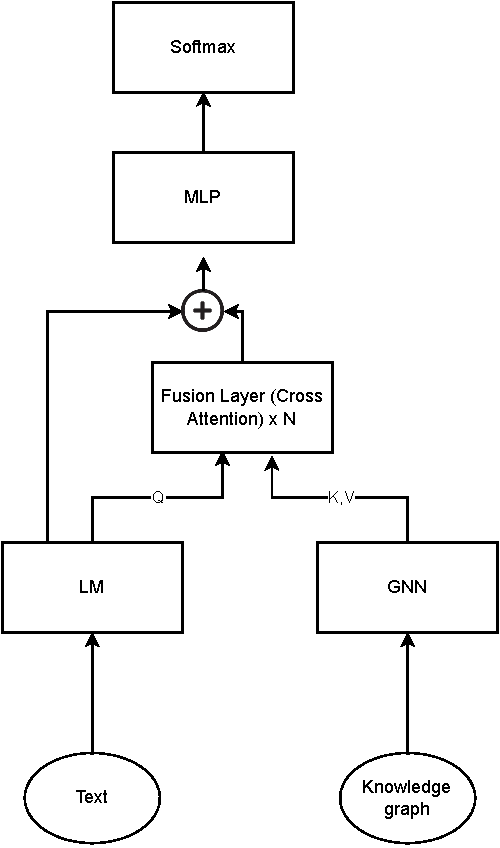
\includegraphics[width=0.6\linewidth]{experiements/image/proposal.pdf}
    \caption{Proposal of Fusion architecture}
    \label{fig:p_proposal}
\end{figure}

% Based on the above results

% Figure \ref{fig:p_rag} illustrated the pipeline of Retrieval-augmented generation. It include \textit{Latent projection}, \textit{Retrieval}, \textit{Context pruning}, \textit{Generator}
% \subsection{Preprocessing data}
% Commonsense corpus includes 20 million sentences \cite{yu2022retrieval}
% Each document is encoded by using bi encoder to build vector database
% \subsection{Generator}
% In this project, Llama-2 is used to perform the generation task, it answers based on the given context. The setting prompt is mentioned in appendix \ref{apd:A}
% \subsection{Latent projection}
% Using text embedding, bi encoder to encode query
% \subsection{Retrieval}
% Using cosine similarity to compare between documents in vector database and embedding vector of query
% Select top-K documents based on similarity score
% \subsection{Context pruning}
% Cross-encoder is employed to make comparison between query and each top-K document, and after that top-K' extract for final contexts
% These context pass to generator to answer the the query from user

Based on the above results, especially Llama-2 KG-RAG, knowledge graph is proposed to use as knowledge base and also to integrate the end-to-end pipeline between knowledge graph and generator. The proposed deep learning model architecture is illustrated in Figure \ref{fig:p_proposal}. In this architecture, a graph encoder extracts the main features of sub-knowledge graph. This graph encoder employs Graph Neural Network \cite{4700287}. The Fusion layer fuses the word embedding from Large Language Model and the list entity embedding from graph encoder using self-attention mechanism. The word embedding from large language model is then concatenated with the extracted feature output from Fusion layer along the feature dimension. Finally, the position-wise Multi-layer Perceptron (MLP) and softmax are applied to obtain the vocabulary distribution for generating the next word.\\\\
Table \ref{tab:effect_kg} shows that effective subgraph retrieval and appropriate training strategy are essential to align the generator’s behavior. Due to the time and resource constraints, the proposal is not completed, still in experimenting. The next project will consider the effectiveness of message passing in graph encoder to exploit the entity and edge in knowledge graph, the training strategy, and the subgraph retrieval.